\chapter{Xây dựng giải pháp \tenKL}

\section{Mô tả giải pháp}

\subsection{Mô tả yêu cầu hệ thống}

Để hỗ trợ việc hiện thực hóa các mục tiêu nghiên cứu, cần có một hệ thống được thiết kế và triển khai nhằm kiểm chứng tính khả thi của các đề xuất kỹ thuật. Phần này sẽ trình bày chi tiết kiến trúc tổng thể, các thành phần chức năng chính, cũng như mối liên kết giữa chúng. Việc mô tả rõ ràng hệ thống không chỉ giúp minh bạch hóa quá trình phát triển mà còn tạo tiền đề cho việc đánh giá hiệu năng và khả năng mở rộng trong các phần sau.

\begin{figure}[htbp]
    \centering
    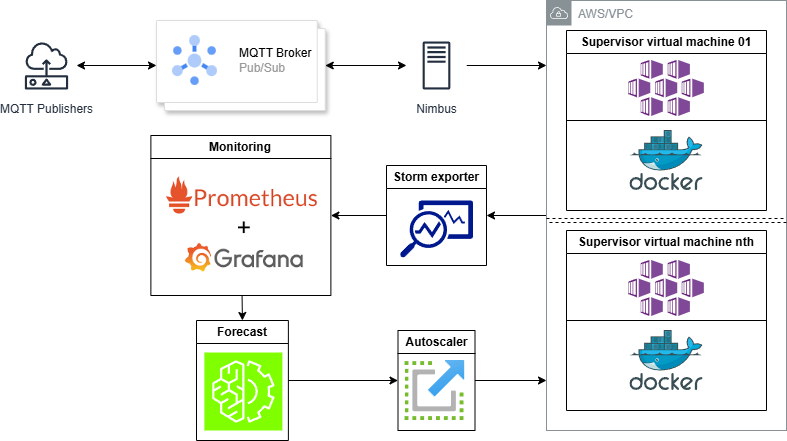
\includegraphics[width=\textwidth]{deployment-architect.drawio.png}
    \caption{Sơ đồ kiến trúc của hệ thống dựa báo và co dãn tài nguyên trên môi trường điện toán đám mây}
\end{figure}

Các thành phần của hệ thống:

\begin{itemize}
    \item MQTT Publisher và Broker có vai trò gửi và chuyển các gói tin (dữ liệu nhà thông minh) đến các subscriber.
    \item Cụm Apache Storm gồm:
          \begin{itemize}
              \item Nimbus và Zookeeper điều phối và chỉ đạo các Supervisor.
              \item Supervisor chạy trong Docker container tại các máy ảo trên nền tảng cloud xử lý dữ liệu.
          \end{itemize}
    \item Storm exporter chịu trách nhiệm thu thập dữ liệu topology và các chỉ số của Docker.
    \item Prometheus thu thập dữ liệu chỉ số từ Storm exporter, Grafana có nhiệm vụ trực quan hóa các chỉ số này.
    \item Storm forecast lấy các chỉ số từ Prometheus để dự đoán tài nguyên co dãn.
    \item Storm autoscaler co dãn tài nguyên máy ảo/container.
\end{itemize}

Luồng dữ liệu sẽ thực hiện tuần tự như sau:

\begin{enumerate}
    \item Dữ liệu từ các thiết bị trong nhà thông minh được thu thập bởi MQTT publisher sau đó được gửi đến MQTT broker. MQTT broker nhận dữ liệu và phân phối chúng đến các subscriber.
    \item Cụm Storm có các spout đóng vai trò subscriber nhận dữ liệu này và tiến hành xử lý dữ liệu. Do lượng dữ liệu trong hệ thống nhà thông minh không đồng đều tại các thời điểm khác, tài nguyên hệ thống cần để đảm bảo xử lý dữ liệu kịp thời đáp ứng nhu cầu tải công việc cũng sẽ thay đổi.
    \item Storm exporter sẽ định kỳ thu thập các chỉ số từ các Supervisor thông qua Storm UI \acrshort{api} và Docker \acrshort{api}.
    \item Prometheus sẽ theo định kỳ thu thập các chỉ số từ Storm exporter để lưu trữ và phục vụ truy vấn.
    \item Grafana sẽ lấy nguồn dữ liệu từ Prometheus để trực quan hóa các chỉ số, hỗ trợ công việc vận hành, phân tích dữ liệu trực quan sau này và cung cấp cái nhìn tổng quát về hệ thống co dãn.
    \item Storm forecast thu thập các chỉ số từ Prometheus thông qua PromQL, tiến hành dự đoán tài nguyên co dãn Supervisor.
    \item Storm autoscaler tiến hành co dãn tài nguyên Supervisor/máy ảo dựa trên chỉ thị của Storm forecast, sau đó autoscaler chờ 10 giây trước khi yêu cầu nimbus thực hiện lệnh tái phân phối (rebalance) các tiến trình.
\end{enumerate}

\subsubsection{Phương án triển khai}

Trong quá trình thiết kế hệ thống tự động co dãn tài nguyên dựa trên học tăng cường, hai hướng triển khai thuật toán Q-learning thường được cân nhắc: (1) huấn luyện trực tiếp trong môi trường (online learning) và (2) chia tách thành hai giai đoạn huấn luyện – đánh giá (offline learning). Phương pháp học trực tiếp cho phép agent liên tục cập nhật chính sách dựa trên tương tác thực tế, từ đó thích nghi tốt với những thay đổi động của môi trường. Tuy nhiên, thời gian để học được một chính sách tốt có thể mất nhiều thời gian, nhất là với môi trường lớn/phức tạp như điện toán đám mây.

Ngược lại, offline learning sử dụng dữ liệu lịch sử hoặc mô phỏng để huấn luyện trước một chính sách ban đầu, từ đó đảm bảo an toàn và kiểm soát tốt hơn quá trình học. Tuy nhiên, chính sách học được có thể thiếu tính linh hoạt trong các kịch bản chưa từng xuất hiện trong tập dữ liệu. Đặc biệt trong bài toán mà đề án này nghiên cứu hoạt động trên môi trường điện toán đám mây, có rất nhiều yếu tố ngoại cảnh sẽ ảnh hưởng đến hệ thống.

Vì vậy, để cân bằng giữa độ an toàn và khả năng thích ứng, luận văn sử dụng phương án kết hợp (hybrid): trước hết huấn luyện offline từ hệ thống mô phỏng, sau đó fine-tune chính sách thông qua học online trong môi trường điện toán đám mây. Cách tiếp cận này tận dụng ưu điểm của cả hai phương pháp, giúp hệ thống đạt hiệu quả co dãn cao mà vẫn đảm bảo tính ổn định trong vận hành thực tế.

\subsubsection{Yêu cầu của hệ thống:}

\begin{itemize}
    \item Cân bằng giữa việc mở rộng và thu hẹp: Đảm bảo không mở rộng quá mức khi hệ thống có chịu được tải, do môi trường triển khai trên hệ thống điện đoán đám mây, bất kỳ tài nguyên không hợp lý nào đều sẽ gây ra lãng phí. Không thu hẹp quá nhiều khiến hệ thống thiếu tài nguyên xử lý, gây ảnh hưởng nghiêm trọng đến trải nghiệm người dùng.
    \item Hiệu năng ổn định: Hệ thống hoạt động ổn định, xuyên suốt.
    \item Tự động cấu hình lại tài nguyên: Hệ thống cần có khả năng tự động cấu hình lại các tài nguyên như máy chủ ảo hoặc container mà không cần sự can thiệp thủ công.
    \item Giám sát hiệu suất: Hệ thống phải có khả năng theo dõi liên tục các chỉ số như CPU, bộ nhớ, băng thông mạng và độ trễ.
\end{itemize}

\section{Xây dựng mô hình học tăng cường}

% \begin{center}
%     \begin{figure}[htbp]
%         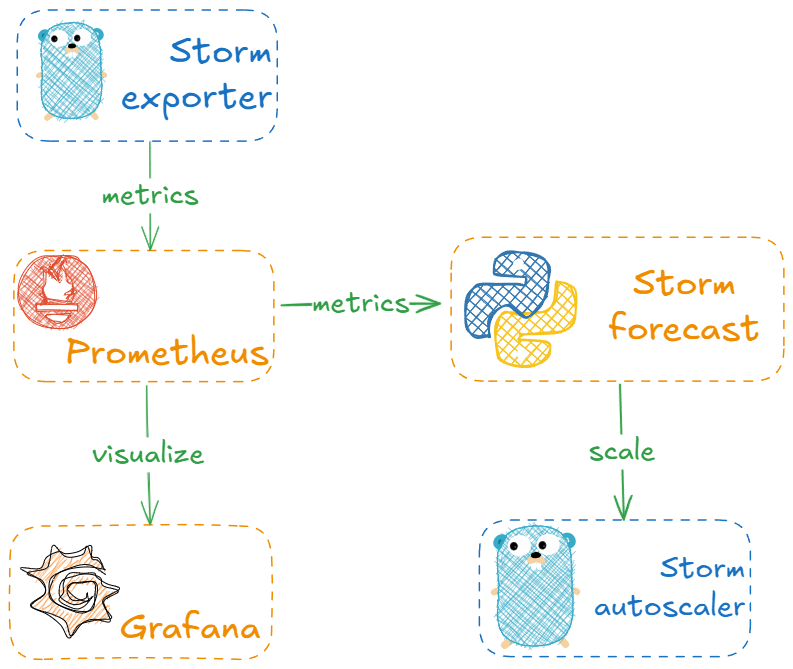
\includegraphics[max width=0.7\textwidth, max height=\textheight]{system-design.png}
%         \caption{Sơ đồ luồng hoạt động của bộ chương trình co dãn}
%     \end{figure}
% \end{center}

\subsection{Mô tả chương trình}

% Dữ liệu chỉ số từ Storm Exporter được Prometheus định kỳ thu thập và lưu trữ. Storm forecast sẽ truy vấn dữ liệu này và dùng chúng để dự đoán tài nguyên cho tương lai, thực hiện co dãn, đánh giá hiệu quả. Cụ thể quá trình này như sau:

% \begin{itemize}
%     \item Storm forecast đọc các chỉ số của supervisor từ Prometheus. Dữ liệu này sau đó được chuyển thành trạng thái trong môi trường học tăng cường thông qua quá trình biến đổi sẽ được trình bày tại thuật toán.
%     \item Storm forecast lựa chọn hành động khám phá (explore) hoặc khai thác (exploit) dựa trên trạng thái hiện tại của môi trường học tăng cường. Sau khi hành động được quyết định, Storm forecast tiến hành yêu cầu Storm autoscaler thực thi quyết định này.
%     \item Storm forecast đọc các chỉ số từ Prometheus và chuyển hóa chúng thành phần thưởng và trạng thái mới của môi trường. Từ các thông tin này, Storm forecast cập nhật hàm giá trị Q.
%     \item Tiến hành lặp lại các bước phía trên đến ngưỡng được định nghĩa thì chương trình dừng lại, tiến hành ghi hàm giá trị Q vào ổ cứng.
%     \item Giai đoạn đánh giá chạy thực nghiệm sẽ sử dụng hàm giá trị Q từ ổ cứng để tiến hành đánh giá. Đồng thời trong quá trình này vẫn tiếp tục cập nhật hàm giá trị Q để đáp ứng các biến đổi về môi trường theo thời gian. Quá trình cập nhật hàm giá trị Q vẫn như trên.
%     \item Storm autoscaler ngoài công việc co/dãn container sẽ tiến hành chuyển hóa các máy ảo với specs nhỏ thành specs lớn hơn để tối ưu chi phí Storm forecast dự án lượng tài nguyên sẽ không thay đổi trong tương lai.
% \end{itemize}

Hệ thống giám sát sử dụng \textit{Prometheus} để thu thập và lưu trữ dữ liệu chỉ số được cung cấp từ \textit{Storm Exporter}. Thành phần \textit{Storm Forecast} sẽ khai thác các dữ liệu này nhằm dự đoán xu hướng sử dụng tài nguyên của các \textit{Supervisor} trong tương lai, từ đó đưa ra quyết định co dãn phù hợp và đánh giá hiệu quả hành động của mình. Toàn bộ quy trình hoạt động được mô tả theo các bước như sau:

\begin{itemize}
    \item \textit{Storm Forecast} truy xuất các chỉ số hoạt động của Supervisor từ Prometheus. Các chỉ số thu được sẽ trải qua quá trình xử lý nhằm chuyển đổi thành biểu diễn trạng thái của môi trường học tăng cường, làm cơ sở cho việc ra quyết định.

    \item Dựa trên trạng thái hiện tại, tác nhân học tăng cường trong \textit{Storm Forecast} sẽ chọn lựa hành động theo chính sách cân bằng giữa khám phá (exploration) và khai thác (exploitation). Sau khi hành động được xác định, hệ thống chuyển tiếp lệnh đến \textit{Storm Autoscaler} để thực hiện. \textit{Storm Autoscaler} sau khi tiến hành co/dãn số lượng supervisor và đợi 10 giây sẽ yêu cầu \textit{Storm Nimbus}

    \item Sau khi hành động được áp dụng, các chỉ số hệ thống tiếp tục được cập nhật thông qua Prometheus. Những dữ liệu mới này sẽ được phân tích để xác định phần thưởng nhận được, đồng thời thiết lập trạng thái tiếp theo của môi trường. Các thông tin này giúp điều chỉnh và cập nhật hàm giá trị \( Q \), từ đó cải thiện chất lượng quyết định trong tương lai.

    \item Chu trình huấn luyện được lặp lại liên tục cho đến khi đạt tới số vòng lặp hoặc điều kiện dừng đã định trước. Khi kết thúc giai đoạn huấn luyện, hàm giá trị \( Q \) sẽ được lưu trữ trên ổ đĩa để phục vụ cho các giai đoạn đánh giá tiếp theo.

    \item Trong giai đoạn đánh giá, hệ thống sử dụng hàm \( Q \) đã học được để đưa ra quyết định, điều này giúp giảm thiểu chi phí thiệt hại so với việc để tác nhân học từ đầu trên môi trường thực. Để đảm bảo khả năng thích nghi với biến động của môi trường, việc cập nhật hàm \( Q \) vẫn được tiếp tục diễn ra.

          % \item Ngoài chức năng co/dãn container, \textit{Storm Autoscaler} còn thực hiện điều chỉnh cấu hình máy ảo - chẳng hạn nâng cấp từ loại máy ảo với thông số kỹ thuật thấp lên loại cao hơn - khi hệ thống dự đoán rằng nhu cầu tài nguyên sẽ ổn định, từ đó tối ưu chi phí vận hành.
\end{itemize}

\subsection{Đầu vào của Storm forecast}

Mỗi trạng thái trong môi trường được biểu thị bởi ba tham số:

\begin{enumerate}
    \item Trung bình tỷ lệ sử dụng bộ nhớ của toàn bộ các supervisor.
    \item Tổng số lượng gói tin các spout gửi đi.
    \item Số lượng supervisor hiện tại.
\end{enumerate}

Các tham số được truy vấn và tính trung bình trong khoảng thời gian 20 giây gần nhất để tránh các trường hợp tham số có giá trị cao hoặc thấp đột biến gây sai lệch trong việc đánh giá.

Trong Q-learning, trạng thái và hành động đều cần ở dạng rời rạc để làm chỉ số cho bảng Q. Khi trạng thái có dạng liên tục, không thể lưu trữ đầy đủ mọi giá trị vào bảng, dẫn đến không thể tra cứu hoặc cập nhật chính xác. Để giải quyết vấn đề này, người ta thường áp dụng kỹ thuật state discretization (tạm dịch: phân rời hóa trạng thái).

\begin{figure}[htbp]
    \centering
    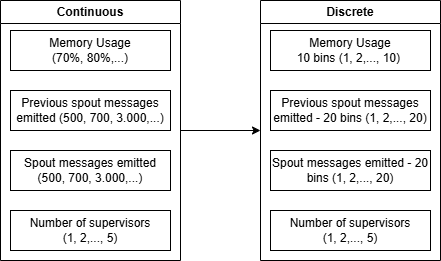
\includegraphics{flows-state-discretization.drawio.png}
    \caption{Sơ đồ minh họa phân rời hóa trạng thái}
\end{figure}

\subsection{Hàm đánh giá giá trị của hành động}

Giá trị của mỗi hành động được đánh giá bởi bốn tham số thu được trong trạng thái kế tiếp.

\paragraph{Trung bình tỷ lệ sử dụng bộ nhớ}

Một yếu tố quan trọng đầu tiên cần được xem xét là trung bình tỷ lệ sử dụng bộ nhớ của toàn bộ các supervisor trong khoảng thời gian 20 giây gần nhất. Mức phạt liên quan đến yếu tố này được đánh giá dựa trên hai kịch bản cụ thể.

Thứ nhất, nếu số lượng supervisor đã đạt đến mức tối thiểu và tỷ lệ sử dụng bộ nhớ trung bình của tất cả các supervisor vẫn thấp hơn ngưỡng mục tiêu đã định (trong nghiên cứu này là 60\%), thì mức phạt sẽ được gán là 0. Điều này là do đây được xác định là một hành động tối ưu, khi hệ thống đang hoạt động với số lượng tài nguyên ít nhất có thể mà vẫn đảm bảo hiệu suất dưới mức tải cho phép.

Thứ hai, trong tất cả các trường hợp còn lại, hình phạt sẽ được tính bằng độ lệch giữa tỷ lệ sử dụng bộ nhớ thực tế đo được và tỷ lệ sử dụng bộ nhớ mong muốn (60\%) cộng với hình phạt nặng khi tỷ lệ sử dụng bộ nhớ vượt quá các ngưỡng, cụ thể là trên 80\% và dưới 20\%.

\paragraph{Hình phạt chi phí vận hành}

Bên cạnh việc tối ưu hóa việc sử dụng bộ nhớ, tác nhân còn phải đối mặt với hình phạt chi phí vận hành. Nguyên tắc cơ bản của hình phạt này là số lượng supervisor càng lớn thì chi phí vận hành càng cao, và do đó, hình phạt càng lớn. Điều này khuyến khích tác nhân ưu tiên sử dụng ít tài nguyên hơn khi có thể, nhằm giảm thiểu chi phí liên quan đến việc duy trì và quản lý một số lượng lớn các supervisor. Hình phạt này là một hàm tuyến tính dựa vào số lượng supervisor hiện tại so với số lượng supervisor tối đa được quy định. Mục tiêu là tạo ra sự cân bằng giữa việc đảm bảo hiệu suất hệ thống (thông qua việc sử dụng đủ supervisor khi cần) và việc tối thiểu hóa chi phí vận hành (bằng cách giảm số lượng supervisor khi có thể mà không ảnh hưởng đến hiệu suất).

\paragraph{Hình phạt độ trễ}

\begin{figure}
    \begin{minipage}{0.48 \textwidth}
        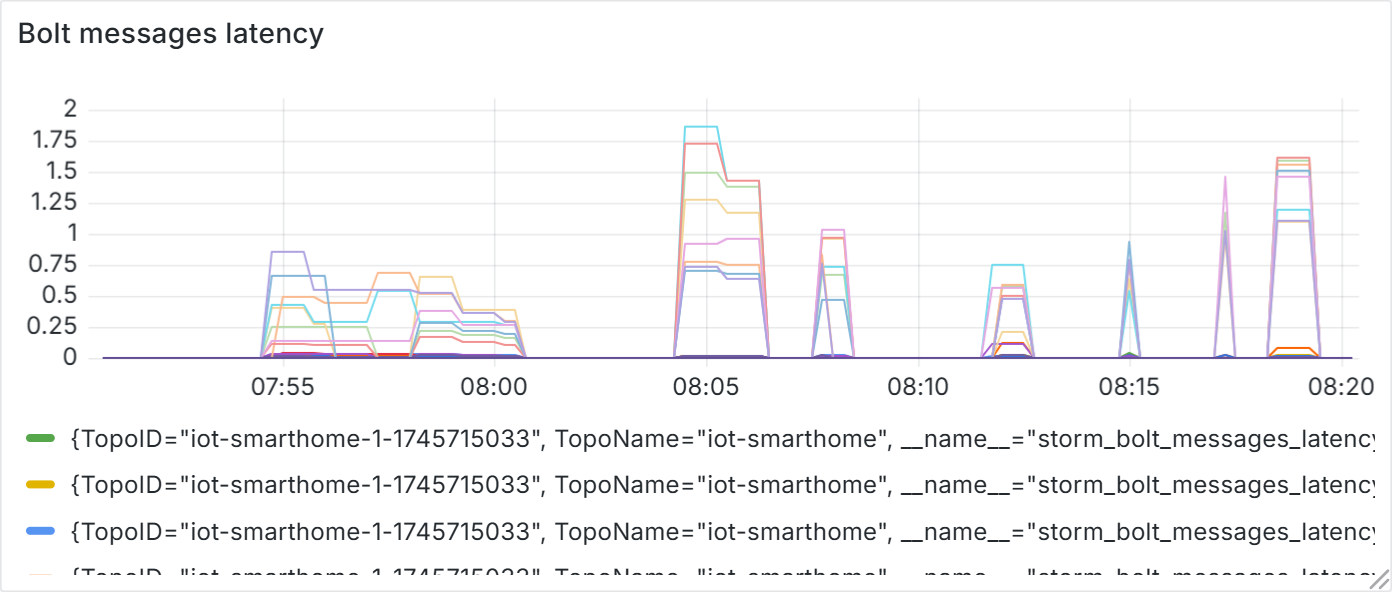
\includegraphics[width=\textwidth]{training-bolt-messages-latency.png}
        \caption{Độ trễ của các bolt trong quá trình huấn luyện}
    \end{minipage}
    \begin{minipage}{0.48 \textwidth}
        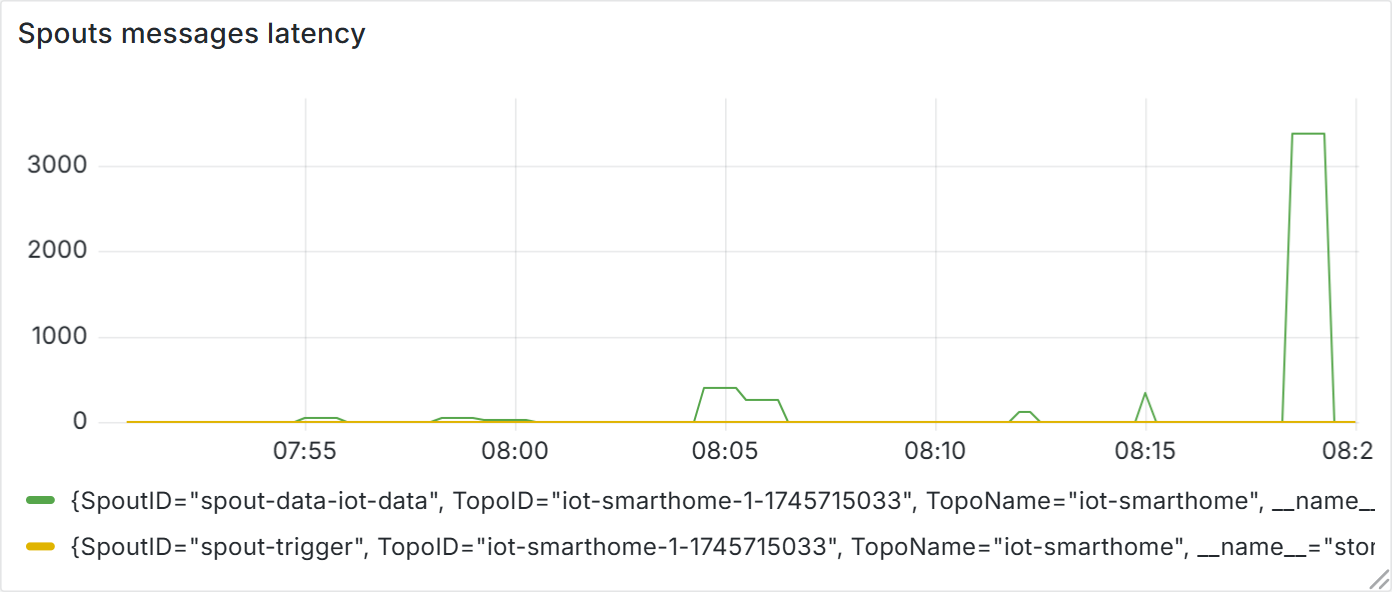
\includegraphics[width=\textwidth]{training-spout-messages-latency.png}
        \caption{Độ trễ của các spout trong quá trình huấn luyện}
    \end{minipage}
\end{figure}

Trong quá trình huấn luyện, tác giả nhận thấy độ trễ của các spout thường lớn hơn đáng kể so với các bolt. Do spout đóng vai trò là nguồn đầu vào dữ liệu cho toàn bộ luồng xử lý, độ trễ cao ở giai đoạn này sẽ ảnh hưởng tiêu cực đến hiệu suất chung của hệ thống. Do đó việc đánh hình phạt cho độ trễ cũng nên được cân nhắc để có thể đảm bảo hệ thống hoạt động với hiệu suất cao, hiệu năng ổn định. Hình phạt này là một hàm tuyến tính dựa trên độ trễ hiện tại của tổng các gói tin của spout.

\paragraph{Thưởng ổn định}

Tác nhân được nhận một phần thưởng nhỏ khi thực hiện hành động không thay đổi số lượng supervisor. Cơ chế này khuyến khích tác nhân duy trì trạng thái hiện tại, hướng đến sự ổn định của cấu trúc topology Storm và giảm thiểu nguy cơ downtime phát sinh do các thay đổi supervisor không cần thiết. Ví dụ, trong tình huống hệ thống đang vận hành với 3 supervisor và tỷ lệ sử dụng bộ nhớ trung bình là 50\%, thay vì thực hiện hành động giảm bớt 1 supervisor (có thể dẫn đến việc 2 supervisor còn lại chịu tải tăng lên đến 75\%), phần thưởng ổn định sẽ tạo động lực để tác nhân ưu tiên giữ nguyên số lượng supervisor hiện có.

\begin{figure}[htbp]
    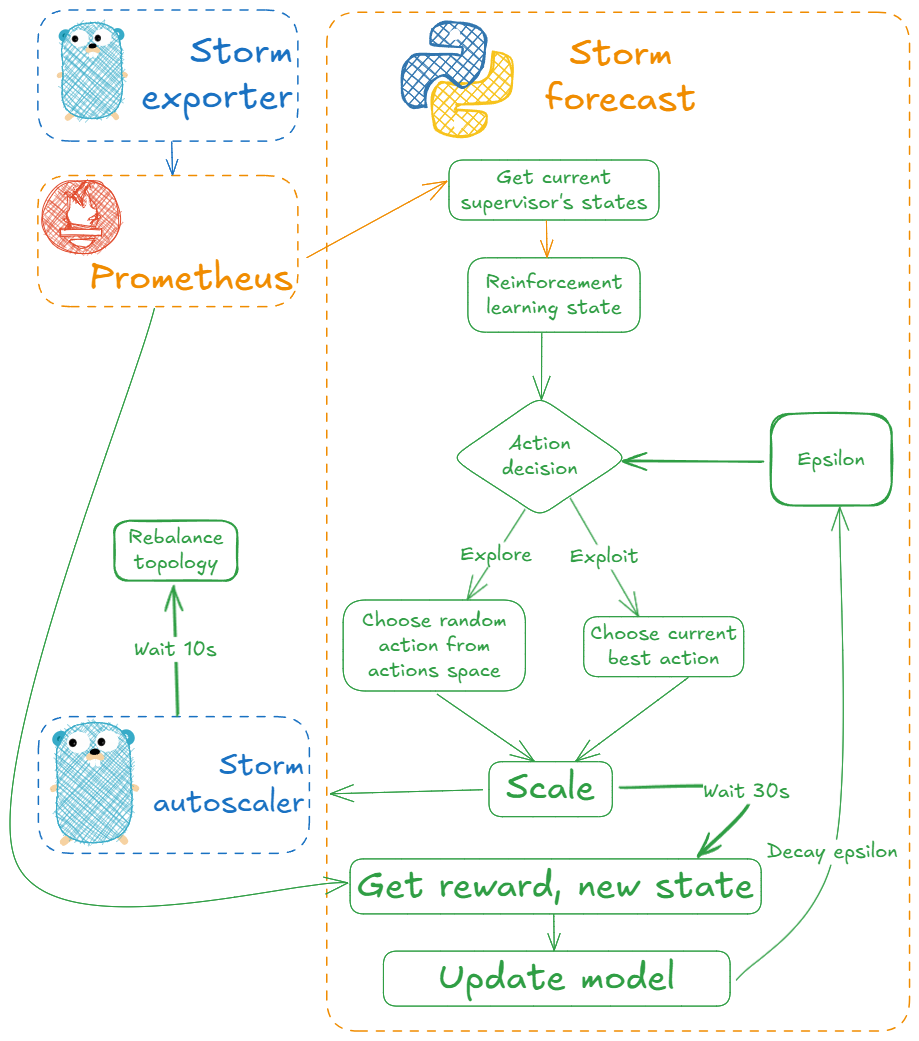
\includegraphics[width=\textwidth]{forecast-workflow.png}
    \caption{Sơ đồ luồng dự đoán tài nguyên}
\end{figure}

\paragraph{Phương trình hàm giá trị}

Dựa trên bốn tham số đã được liệt kê bên trên, tác giả đã xây dựng hàm giá trị $V(a, s')$ cho trạng thái kế tiếp $s'$ có dạng tổng quát như sau:
\begin{equation}
    \begin{split}
        V(a, s') = \omega_{stable} \cdot R_{stable}(a) - \omega_{memory} \cdot P_{memory}(s'_{memory}) \\
        - \omega_{latency} \cdot P_{latency}(s'_{latency}) \omega_{cost} \cdot P_{cost}(s'_{supervisor})
    \end{split}
\end{equation}
trong đó:

\begin{itemize}
    \item $\omega_{stable}$, $\omega_{stable}$, $\omega_{stable}$, $\omega_{latency}$ là các trọng số không âm, thể hiện tầm quan trọng tương đối của từng thành phần trong việc đánh giá.
    \item $R_{stable}(a)$, $P_{memory}(s'_{memory})$, $P_{cost}(s'_{supervisor})$, $P_{latency}(s'_{latency})$ được định nghĩa tương tự như trước.
    \item Dấu (-) trước các hành động thể hiện hình phạt thay vì dùng các trọng số âm sẽ gây phức tạp và dễ nhầm lẫn trong việc điều chỉnh các trọng số.
\end{itemize}

\subsection{Phương án lựa chọn hành động}

Chiến lược lựa chọn hành động $\epsilon$-greedy được áp dụng như sau: tại mỗi bước ra quyết định, tác nhân sẽ tạo một số ngẫu nhiên $r \in [0, 1)$. Hành động được lựa chọn dựa trên sự so sánh giữa $r$ và giá trị $\epsilon$ hiện tại:
\begin{itemize}
    \item Nếu $r < \epsilon$, tác nhân thực hiện một hành động ngẫu nhiên từ tập các hành động khả thi.
    \item Nếu $r \geq \epsilon$, tác nhân lựa chọn hành động có giá trị ước tính cao nhất theo hàm giá trị hiện tại.
\end{itemize}

Trong giai đoạn huấn luyện, giá trị $\epsilon$ ban đầu được thiết lập là $1.0$ và giảm tuyến tính $0.01$ sau mỗi bước cho đến khi đạt ngưỡng tối thiểu là $0.1$. Ngược lại, trong giai đoạn đánh giá, giá trị $\epsilon$ được khởi tạo ở mức $0.1$, tương ứng với giá trị tối thiểu trong quá trình huấn luyện. Giá trị $\epsilon$ này đảm bảo tỷ lệ khai phá (exploration) là $10\%$ trong mỗi 10 lần lựa chọn hành động, tạo điều kiện cho tác nhân thích ứng với những thay đổi tiềm ẩn của môi trường.